% Options for packages loaded elsewhere
\PassOptionsToPackage{unicode}{hyperref}
\PassOptionsToPackage{hyphens}{url}
%
\documentclass[
  ignorenonframetext,
]{beamer}
\usepackage{pgfpages}
\setbeamertemplate{caption}[numbered]
\setbeamertemplate{caption label separator}{: }
\setbeamercolor{caption name}{fg=normal text.fg}
\beamertemplatenavigationsymbolsempty
% Prevent slide breaks in the middle of a paragraph
\widowpenalties 1 10000
\raggedbottom
\setbeamertemplate{part page}{
  \centering
  \begin{beamercolorbox}[sep=16pt,center]{part title}
    \usebeamerfont{part title}\insertpart\par
  \end{beamercolorbox}
}
\setbeamertemplate{section page}{
  \centering
  \begin{beamercolorbox}[sep=12pt,center]{part title}
    \usebeamerfont{section title}\insertsection\par
  \end{beamercolorbox}
}
\setbeamertemplate{subsection page}{
  \centering
  \begin{beamercolorbox}[sep=8pt,center]{part title}
    \usebeamerfont{subsection title}\insertsubsection\par
  \end{beamercolorbox}
}
\AtBeginPart{
  \frame{\partpage}
}
\AtBeginSection{
  \ifbibliography
  \else
    \frame{\sectionpage}
  \fi
}
\AtBeginSubsection{
  \frame{\subsectionpage}
}
\usepackage{lmodern}
\usepackage{amssymb,amsmath}
\usepackage{ifxetex,ifluatex}
\ifnum 0\ifxetex 1\fi\ifluatex 1\fi=0 % if pdftex
  \usepackage[T1]{fontenc}
  \usepackage[utf8]{inputenc}
  \usepackage{textcomp} % provide euro and other symbols
\else % if luatex or xetex
  \usepackage{unicode-math}
  \defaultfontfeatures{Scale=MatchLowercase}
  \defaultfontfeatures[\rmfamily]{Ligatures=TeX,Scale=1}
\fi
% Use upquote if available, for straight quotes in verbatim environments
\IfFileExists{upquote.sty}{\usepackage{upquote}}{}
\IfFileExists{microtype.sty}{% use microtype if available
  \usepackage[]{microtype}
  \UseMicrotypeSet[protrusion]{basicmath} % disable protrusion for tt fonts
}{}
\makeatletter
\@ifundefined{KOMAClassName}{% if non-KOMA class
  \IfFileExists{parskip.sty}{%
    \usepackage{parskip}
  }{% else
    \setlength{\parindent}{0pt}
    \setlength{\parskip}{6pt plus 2pt minus 1pt}}
}{% if KOMA class
  \KOMAoptions{parskip=half}}
\makeatother
\usepackage{xcolor}
\IfFileExists{xurl.sty}{\usepackage{xurl}}{} % add URL line breaks if available
\IfFileExists{bookmark.sty}{\usepackage{bookmark}}{\usepackage{hyperref}}
\hypersetup{
  pdftitle={How to write an R package and publish it on GitHub},
  pdfauthor={Aya Mitani},
  hidelinks,
  pdfcreator={LaTeX via pandoc}}
\urlstyle{same} % disable monospaced font for URLs
\newif\ifbibliography
\usepackage{color}
\usepackage{fancyvrb}
\newcommand{\VerbBar}{|}
\newcommand{\VERB}{\Verb[commandchars=\\\{\}]}
\DefineVerbatimEnvironment{Highlighting}{Verbatim}{commandchars=\\\{\}}
% Add ',fontsize=\small' for more characters per line
\usepackage{framed}
\definecolor{shadecolor}{RGB}{248,248,248}
\newenvironment{Shaded}{\begin{snugshade}}{\end{snugshade}}
\newcommand{\AlertTok}[1]{\textcolor[rgb]{0.94,0.16,0.16}{#1}}
\newcommand{\AnnotationTok}[1]{\textcolor[rgb]{0.56,0.35,0.01}{\textbf{\textit{#1}}}}
\newcommand{\AttributeTok}[1]{\textcolor[rgb]{0.77,0.63,0.00}{#1}}
\newcommand{\BaseNTok}[1]{\textcolor[rgb]{0.00,0.00,0.81}{#1}}
\newcommand{\BuiltInTok}[1]{#1}
\newcommand{\CharTok}[1]{\textcolor[rgb]{0.31,0.60,0.02}{#1}}
\newcommand{\CommentTok}[1]{\textcolor[rgb]{0.56,0.35,0.01}{\textit{#1}}}
\newcommand{\CommentVarTok}[1]{\textcolor[rgb]{0.56,0.35,0.01}{\textbf{\textit{#1}}}}
\newcommand{\ConstantTok}[1]{\textcolor[rgb]{0.00,0.00,0.00}{#1}}
\newcommand{\ControlFlowTok}[1]{\textcolor[rgb]{0.13,0.29,0.53}{\textbf{#1}}}
\newcommand{\DataTypeTok}[1]{\textcolor[rgb]{0.13,0.29,0.53}{#1}}
\newcommand{\DecValTok}[1]{\textcolor[rgb]{0.00,0.00,0.81}{#1}}
\newcommand{\DocumentationTok}[1]{\textcolor[rgb]{0.56,0.35,0.01}{\textbf{\textit{#1}}}}
\newcommand{\ErrorTok}[1]{\textcolor[rgb]{0.64,0.00,0.00}{\textbf{#1}}}
\newcommand{\ExtensionTok}[1]{#1}
\newcommand{\FloatTok}[1]{\textcolor[rgb]{0.00,0.00,0.81}{#1}}
\newcommand{\FunctionTok}[1]{\textcolor[rgb]{0.00,0.00,0.00}{#1}}
\newcommand{\ImportTok}[1]{#1}
\newcommand{\InformationTok}[1]{\textcolor[rgb]{0.56,0.35,0.01}{\textbf{\textit{#1}}}}
\newcommand{\KeywordTok}[1]{\textcolor[rgb]{0.13,0.29,0.53}{\textbf{#1}}}
\newcommand{\NormalTok}[1]{#1}
\newcommand{\OperatorTok}[1]{\textcolor[rgb]{0.81,0.36,0.00}{\textbf{#1}}}
\newcommand{\OtherTok}[1]{\textcolor[rgb]{0.56,0.35,0.01}{#1}}
\newcommand{\PreprocessorTok}[1]{\textcolor[rgb]{0.56,0.35,0.01}{\textit{#1}}}
\newcommand{\RegionMarkerTok}[1]{#1}
\newcommand{\SpecialCharTok}[1]{\textcolor[rgb]{0.00,0.00,0.00}{#1}}
\newcommand{\SpecialStringTok}[1]{\textcolor[rgb]{0.31,0.60,0.02}{#1}}
\newcommand{\StringTok}[1]{\textcolor[rgb]{0.31,0.60,0.02}{#1}}
\newcommand{\VariableTok}[1]{\textcolor[rgb]{0.00,0.00,0.00}{#1}}
\newcommand{\VerbatimStringTok}[1]{\textcolor[rgb]{0.31,0.60,0.02}{#1}}
\newcommand{\WarningTok}[1]{\textcolor[rgb]{0.56,0.35,0.01}{\textbf{\textit{#1}}}}
\setlength{\emergencystretch}{3em} % prevent overfull lines
\providecommand{\tightlist}{%
  \setlength{\itemsep}{0pt}\setlength{\parskip}{0pt}}
\setcounter{secnumdepth}{-\maxdimen} % remove section numbering
\usetheme[progressbar=frametitle]{metropolis}
\usepackage{graphicx}
\usepackage{rotating}
\usepackage{amsmath}
\usepackage{float}
\usefonttheme[onlymath]{serif}
\AtBeginPart{}
\AtBeginSection{}
\AtBeginSubsection{}
\AtBeginSubsubsection{}
\usepackage{multicol}
\newcommand{\btwocol}{\begin{multicols}{2}}
\newcommand{\etwocol}{\end{multicols}}

\title{How to write an R package and publish it on GitHub}
\author{Aya Mitani}
\date{2021/01/07}

\begin{document}
\frame{\titlepage}

\begin{frame}[fragile]{What is R package?}
\protect\hypertarget{what-is-r-package}{}

\begin{itemize}
\tightlist
\item
  Collection of code, data, documentation developed by R community
\item
  Addresses particular problem with specialized statistical technique,
  graphical device, etc.
\item
  Core set of packages come with base R
\item
  \(>\) 15,000 Additional packages available from CRAN, Bioconductor,
  Omegahat, GitHub, etc.
\item
  Popular R packages

  \begin{itemize}
  \tightlist
  \item
    \texttt{dplyr}
  \item
    \texttt{ggplot2}
  \end{itemize}
\end{itemize}

\begin{figure}
  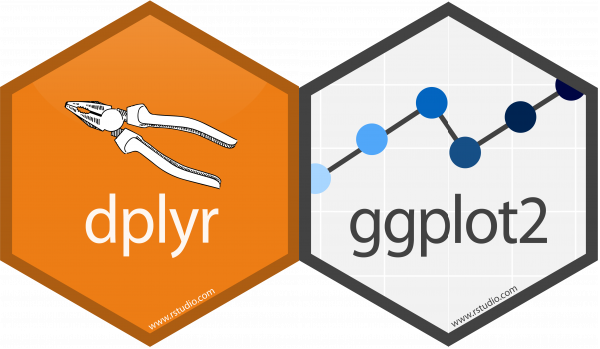
\includegraphics[scale=0.2]{slides_files/figure-beamer/dplyrggplot2.png}
\end{figure}

\end{frame}

\begin{frame}{What is GitHub?}
\protect\hypertarget{what-is-github}{}

\begin{itemize}
\tightlist
\item
  Website that hosts software development and version control using Git
\item
  Free basic services
\end{itemize}

\begin{figure}
  
\includegraphics[scale=0.2]{slides_files/figure-beamer/GitHub.png}
\end{figure}

\end{frame}

\begin{frame}{Why write R package?}
\protect\hypertarget{why-write-r-package}{}

\begin{itemize}
\tightlist
\item
  For yourself
\item
  For others

  \begin{itemize}
  \tightlist
  \item
    Increasingly, (bio)statistical journals ask for R package
    development of novel method
  \end{itemize}
\end{itemize}

\end{frame}

\begin{frame}{Why publish package on GitHub?}
\protect\hypertarget{why-publish-package-on-github}{}

\begin{itemize}
\tightlist
\item
  Reproducibility
\item
  Accessibility
\item
  Collaboration
\item
  Back-up method
\end{itemize}

\end{frame}

\begin{frame}[fragile]{What do you need to write R package?}
\protect\hypertarget{what-do-you-need-to-write-r-package}{}

\begin{itemize}
\tightlist
\item
  R Studio (\url{https://rstudio.com/})
\item
  \texttt{devtools} package
\item
  Git (\url{https://git-scm.com/})
\item
  GitHub account (\url{https://github.com/})
\end{itemize}

\textcolor{blue}{Some other useful packages}

\begin{itemize}
\tightlist
\item
  \texttt{here}
\item
  \texttt{available}
\end{itemize}

\begin{figure}
  \includegraphics[scale=0.2]{slides_files/figure-beamer/Rstudio.png}
\end{figure}

\end{frame}

\begin{frame}[fragile]{Let's begin!}
\protect\hypertarget{lets-begin}{}

\textbf{Major steps}

\begin{enumerate}
\tightlist
\item
  Create new repo in GitHub

  \begin{enumerate}
  [i)]
  \tightlist
  \item
    Copy URL
  \end{enumerate}
\item
  Open R Studio

  \begin{enumerate}
  [i)]
  \tightlist
  \item
    New Project \(\rightarrow\) Version Control \(\rightarrow\) Git
    \(\rightarrow\) Enter info \(\rightarrow\) Create Project
  \item
    Install \texttt{devtools}
  \item
    Build package
  \end{enumerate}
\item
  Pull + Commit + Push
\item
  Use/share package with \texttt{install\_github()}!
\end{enumerate}

\end{frame}

\begin{frame}{In GitHub}
\protect\hypertarget{in-github}{}

First, log in and go to Repositories

\begin{figure}
  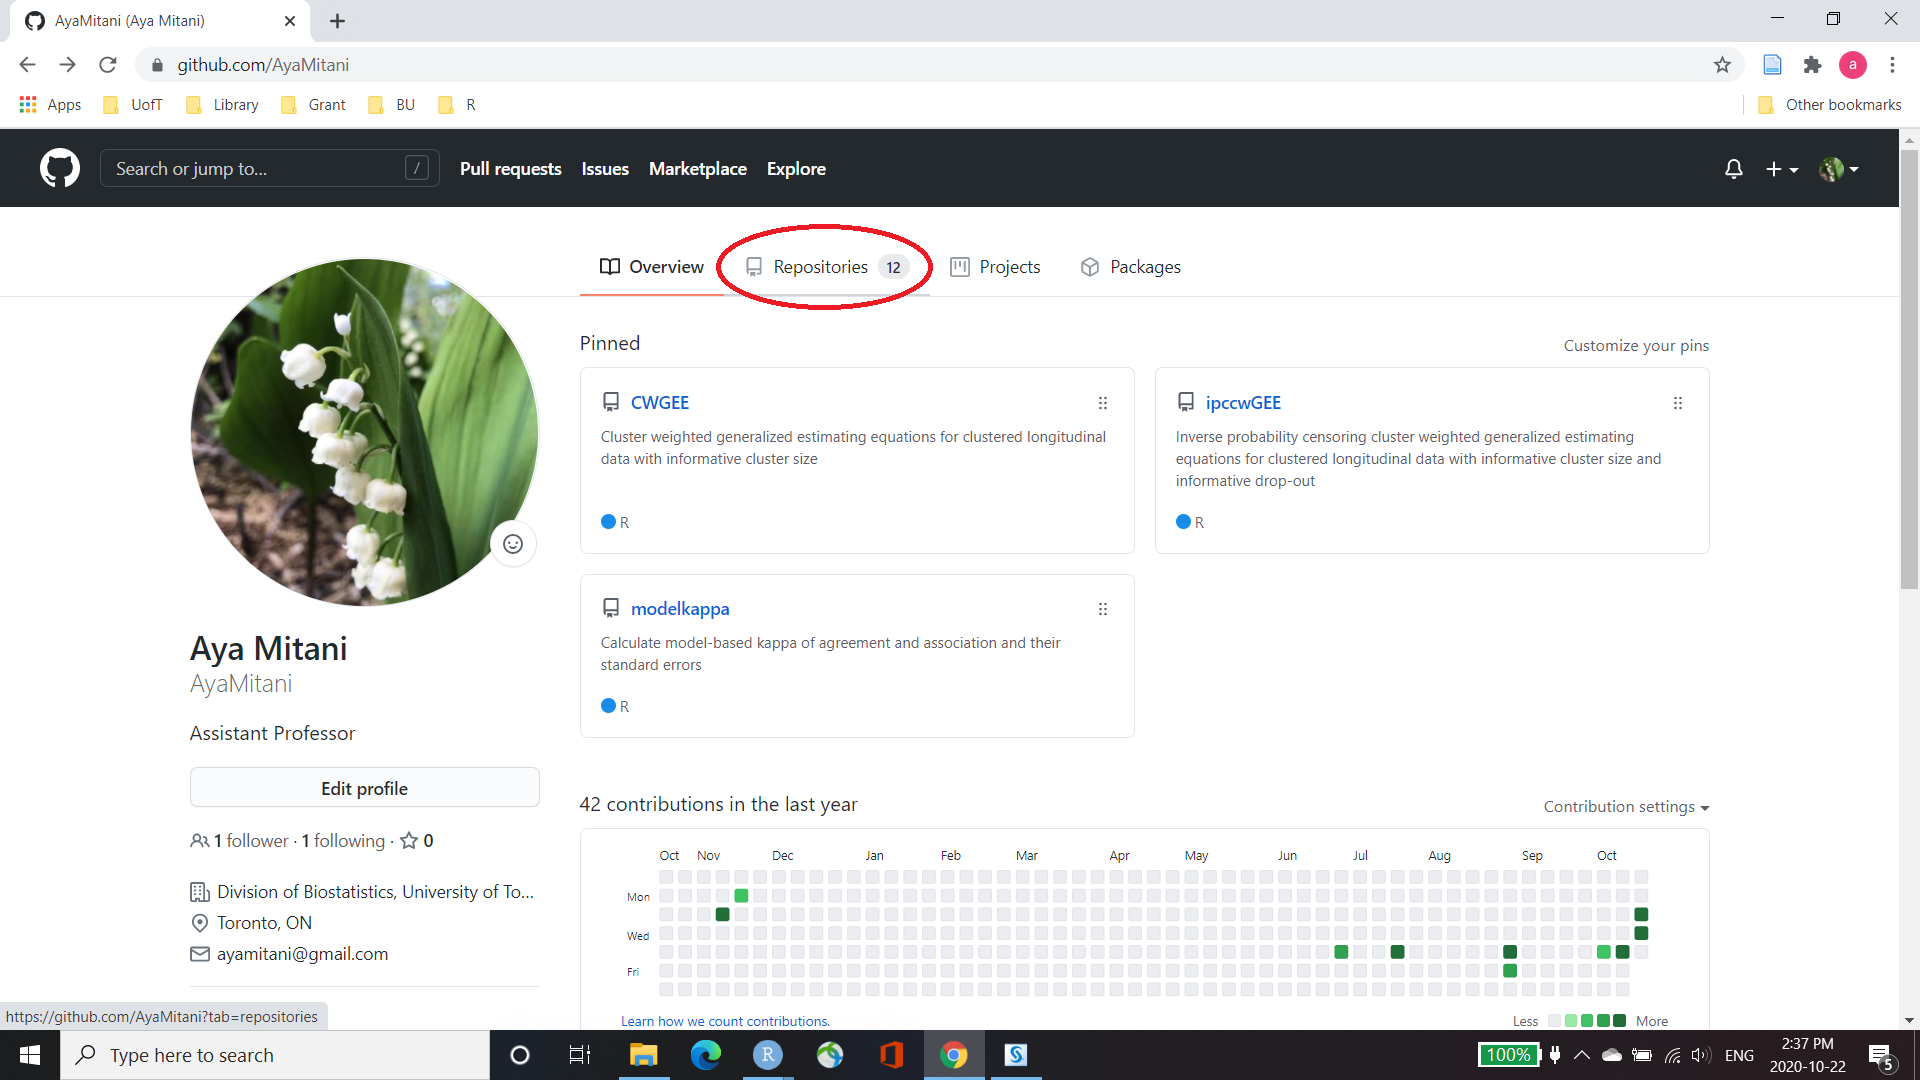
\includegraphics[scale=0.275]{slides_files/figure-beamer/GitHub_step1.png}
\end{figure}

\end{frame}

\begin{frame}{In GitHub}
\protect\hypertarget{in-github-1}{}

Then, create new repository

\begin{figure}
  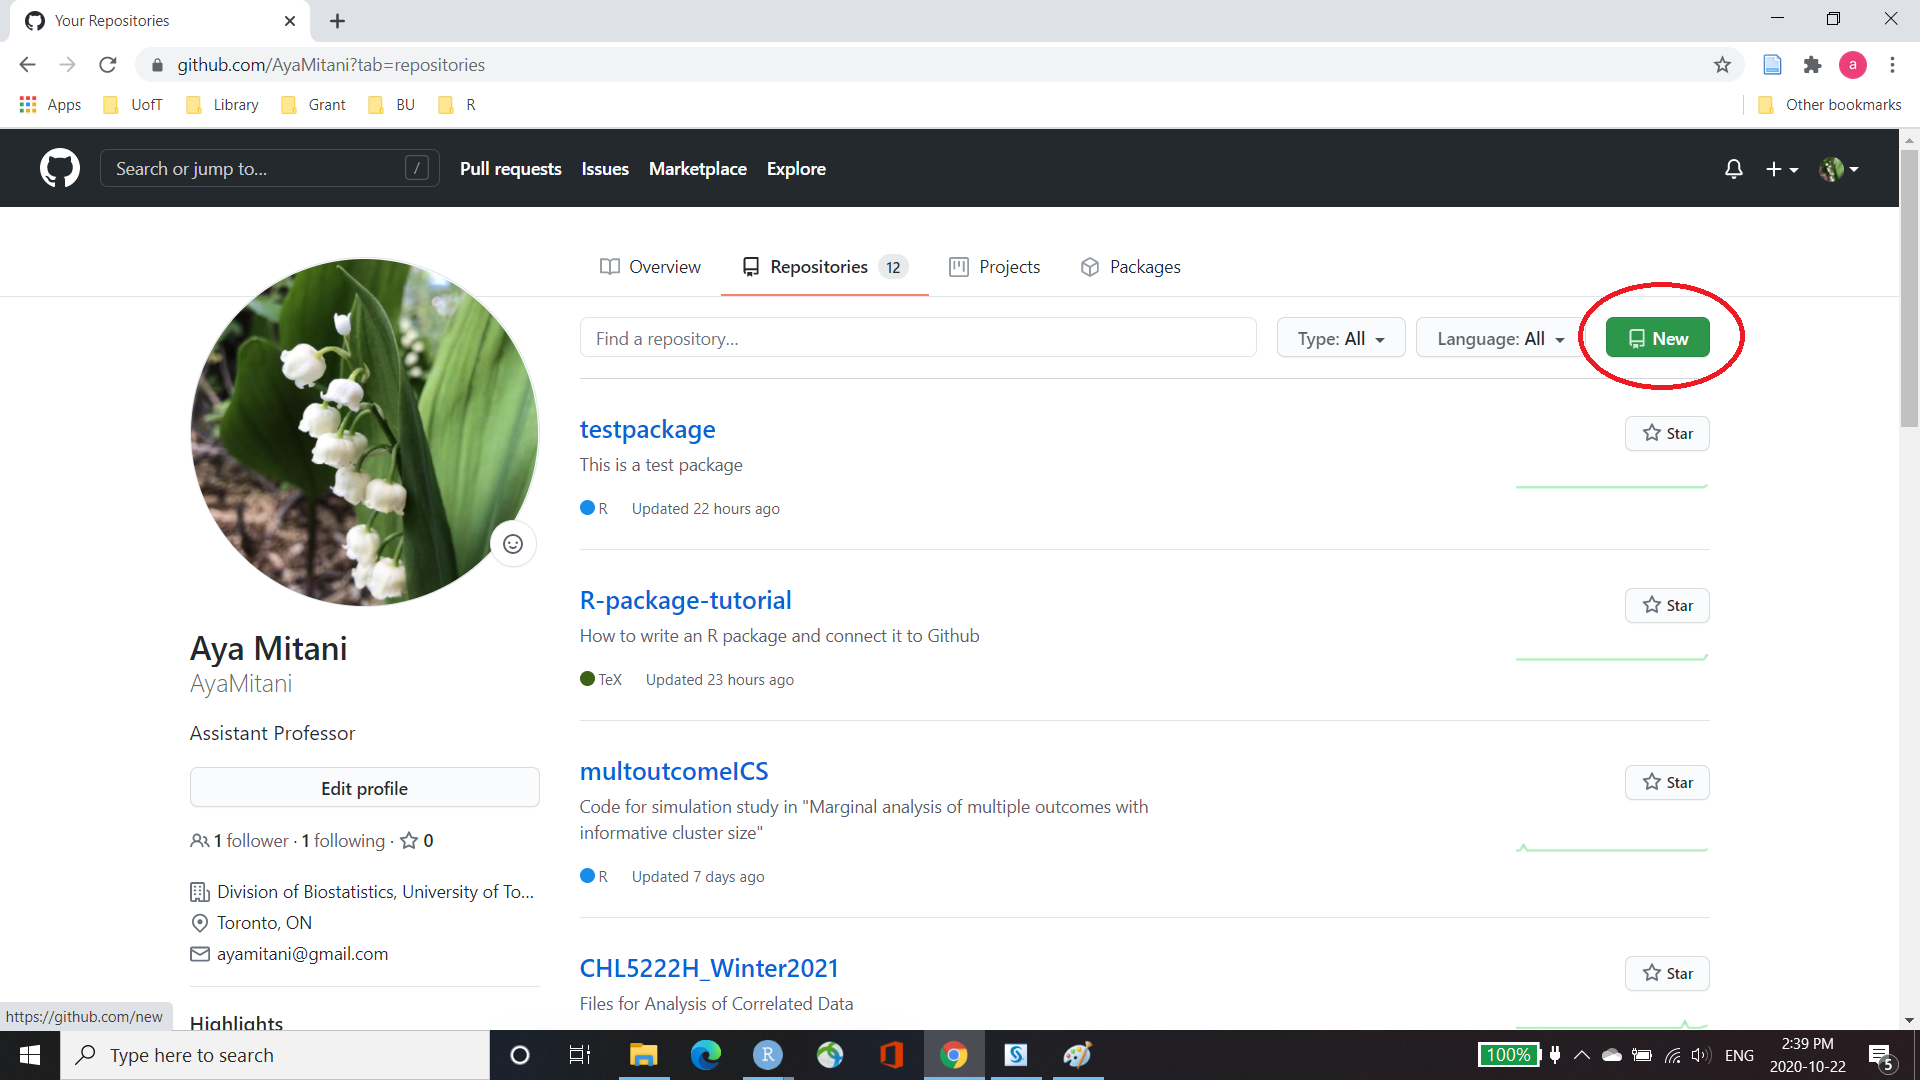
\includegraphics[scale=0.275]{slides_files/figure-beamer/GitHub_step2.png}
\end{figure}

\end{frame}

\begin{frame}{In GitHub}
\protect\hypertarget{in-github-2}{}

Repo name should be same as package name

\begin{figure}
  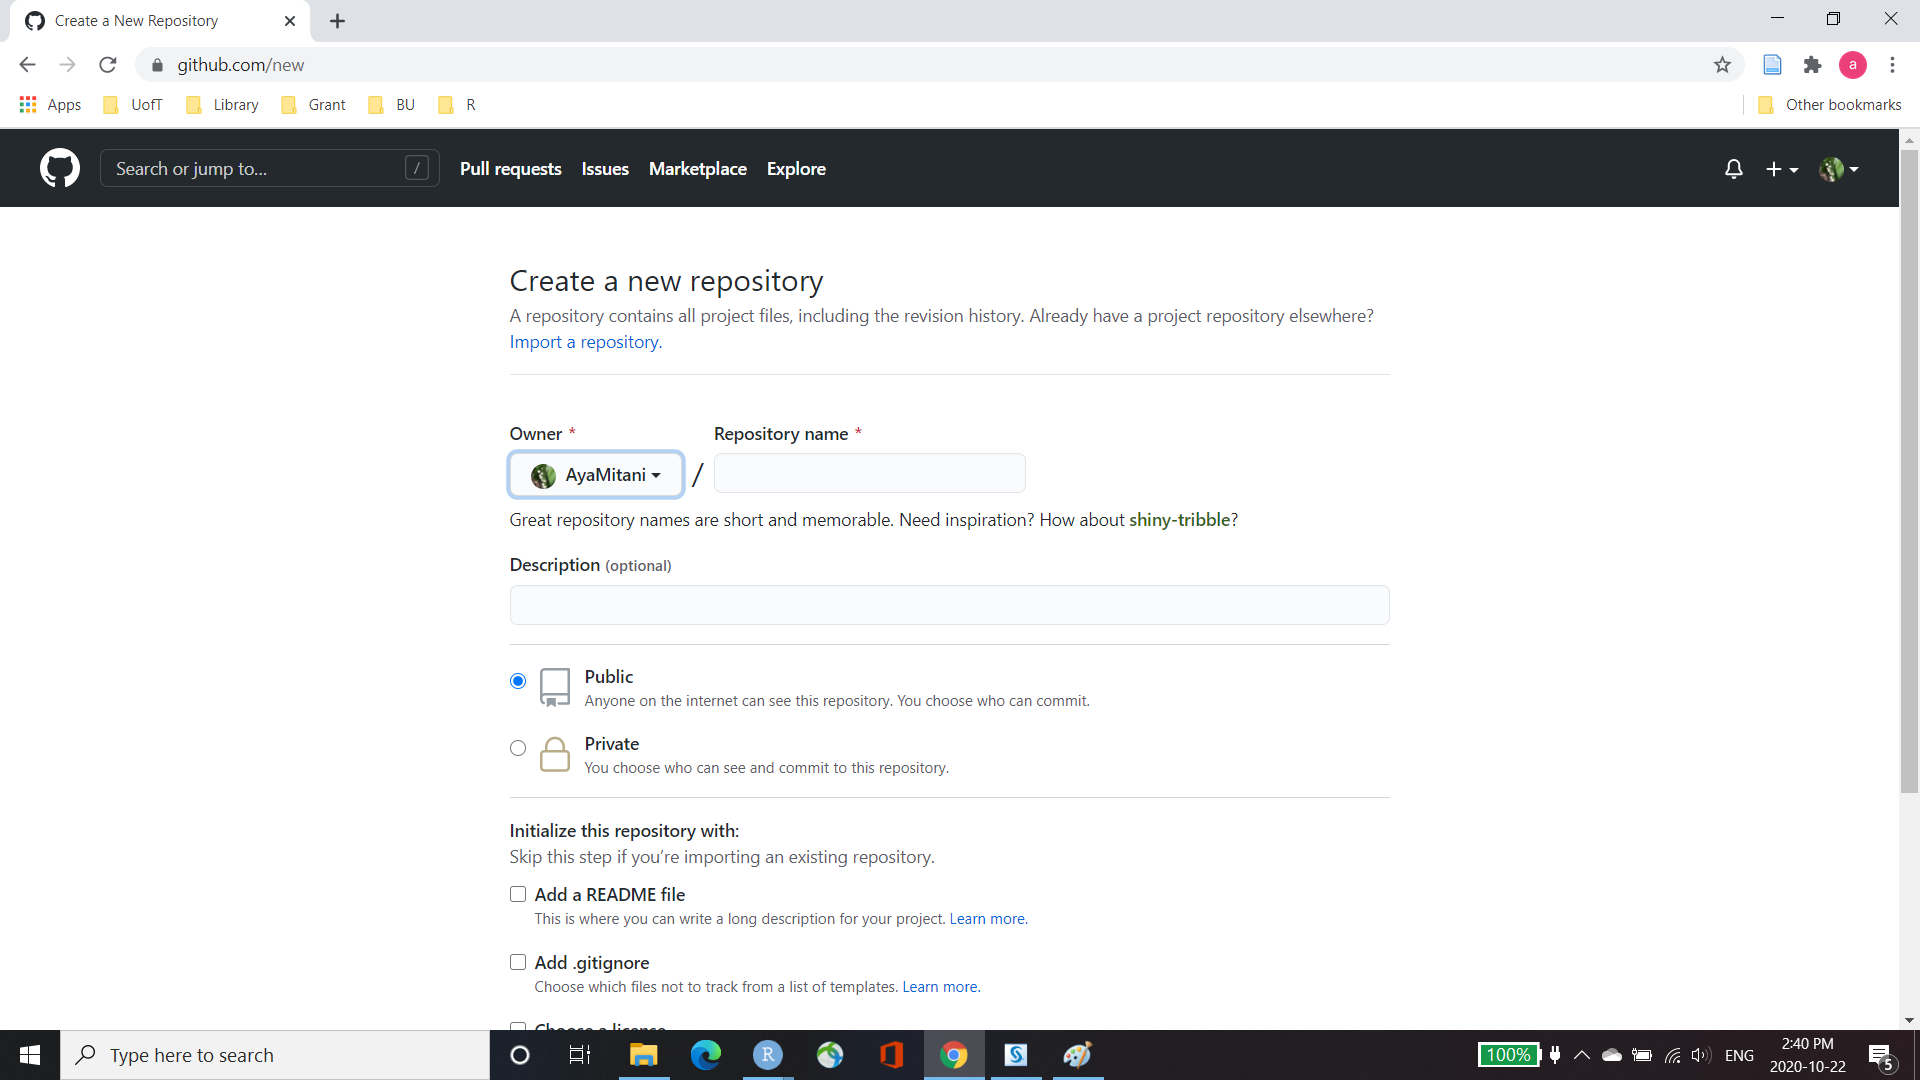
\includegraphics[scale=0.275]{slides_files/figure-beamer/GitHub_step3.png}
\end{figure}

\end{frame}

\begin{frame}[fragile]{Aside: Naming R package}
\protect\hypertarget{aside-naming-r-package}{}

Some tips:

\begin{itemize}
\tightlist
\item
  Make it short
\item
  If one word, use all lowercase
\item
  If multiple words, mix lowercase and uppercase
\item
  Avoid using characters (\texttt{.}, \texttt{\_}) between words
\end{itemize}

\end{frame}

\begin{frame}[fragile]{Aside: Naming R package}
\protect\hypertarget{aside-naming-r-package-1}{}

Check to see if name is unique, especially if you plan to submit to CRAN
\footnotesize

\begin{Shaded}
\begin{Highlighting}[]
\KeywordTok{install.packages}\NormalTok{(}\StringTok{"available"}\NormalTok{)}
\KeywordTok{library}\NormalTok{(available)}
\end{Highlighting}
\end{Shaded}

\begin{Shaded}
\begin{Highlighting}[]
\KeywordTok{available}\NormalTok{(}\StringTok{"ayapack"}\NormalTok{, }\DataTypeTok{browse =} \OtherTok{FALSE}\NormalTok{)}
\end{Highlighting}
\end{Shaded}

\begin{verbatim}
## -- ayapack ---------------------------------------------------------------------
## Name valid: <U+2714>
## Available on CRAN: <U+2714> 
## Available on Bioconductor: <U+2714>
## Available on GitHub:  <U+2714> 
## Abbreviations: http://www.abbreviations.com/ayapack
## Wikipedia: https://en.wikipedia.org/wiki/ayapack
## Wiktionary: https://en.wiktionary.org/wiki/ayapack
## Urban Dictionary:
##   Not found.
## Sentiment:???
\end{verbatim}

\end{frame}

\begin{frame}{Back to GitHub}
\protect\hypertarget{back-to-github}{}

Finish creating new repo

\begin{figure}
  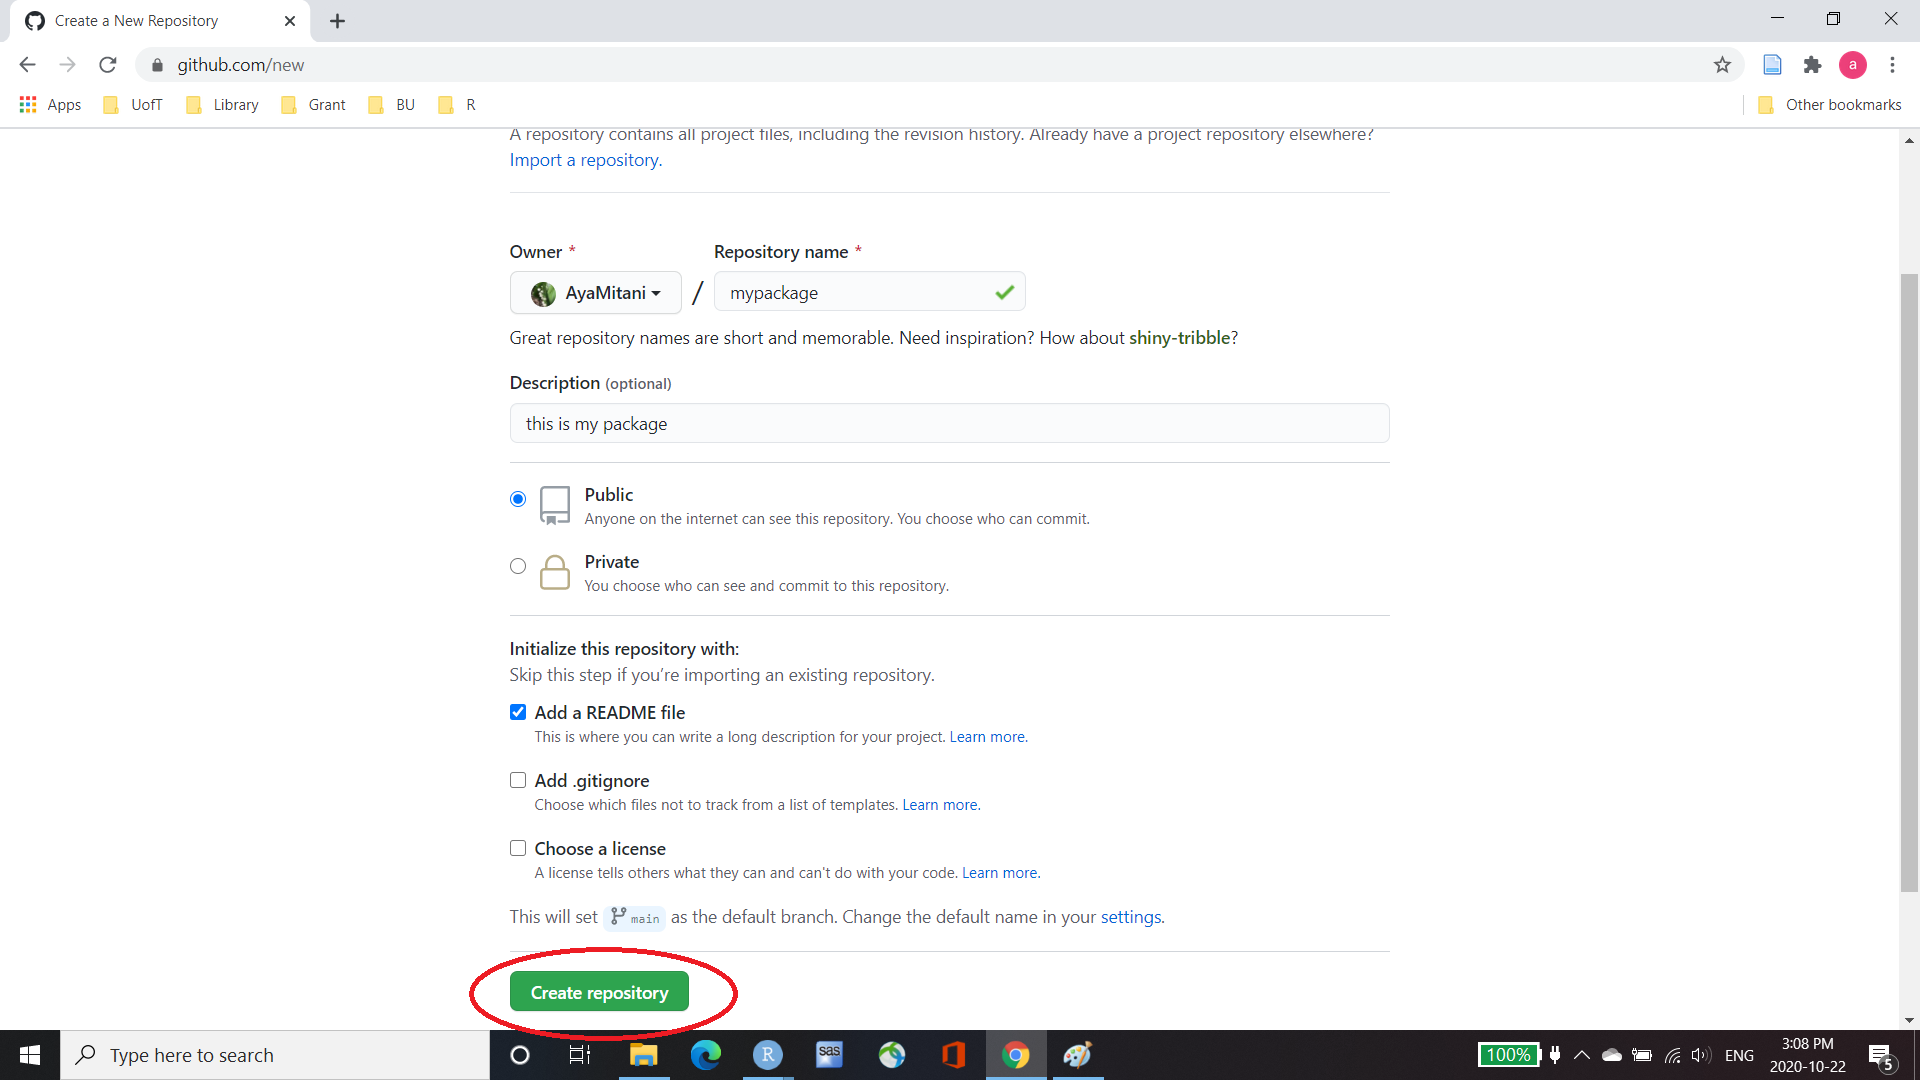
\includegraphics[scale=0.275]{slides_files/figure-beamer/GitHub_step4.png}
\end{figure}

\end{frame}

\begin{frame}{In GitHub}
\protect\hypertarget{in-github-3}{}

Finally, copy URL

\begin{figure}
  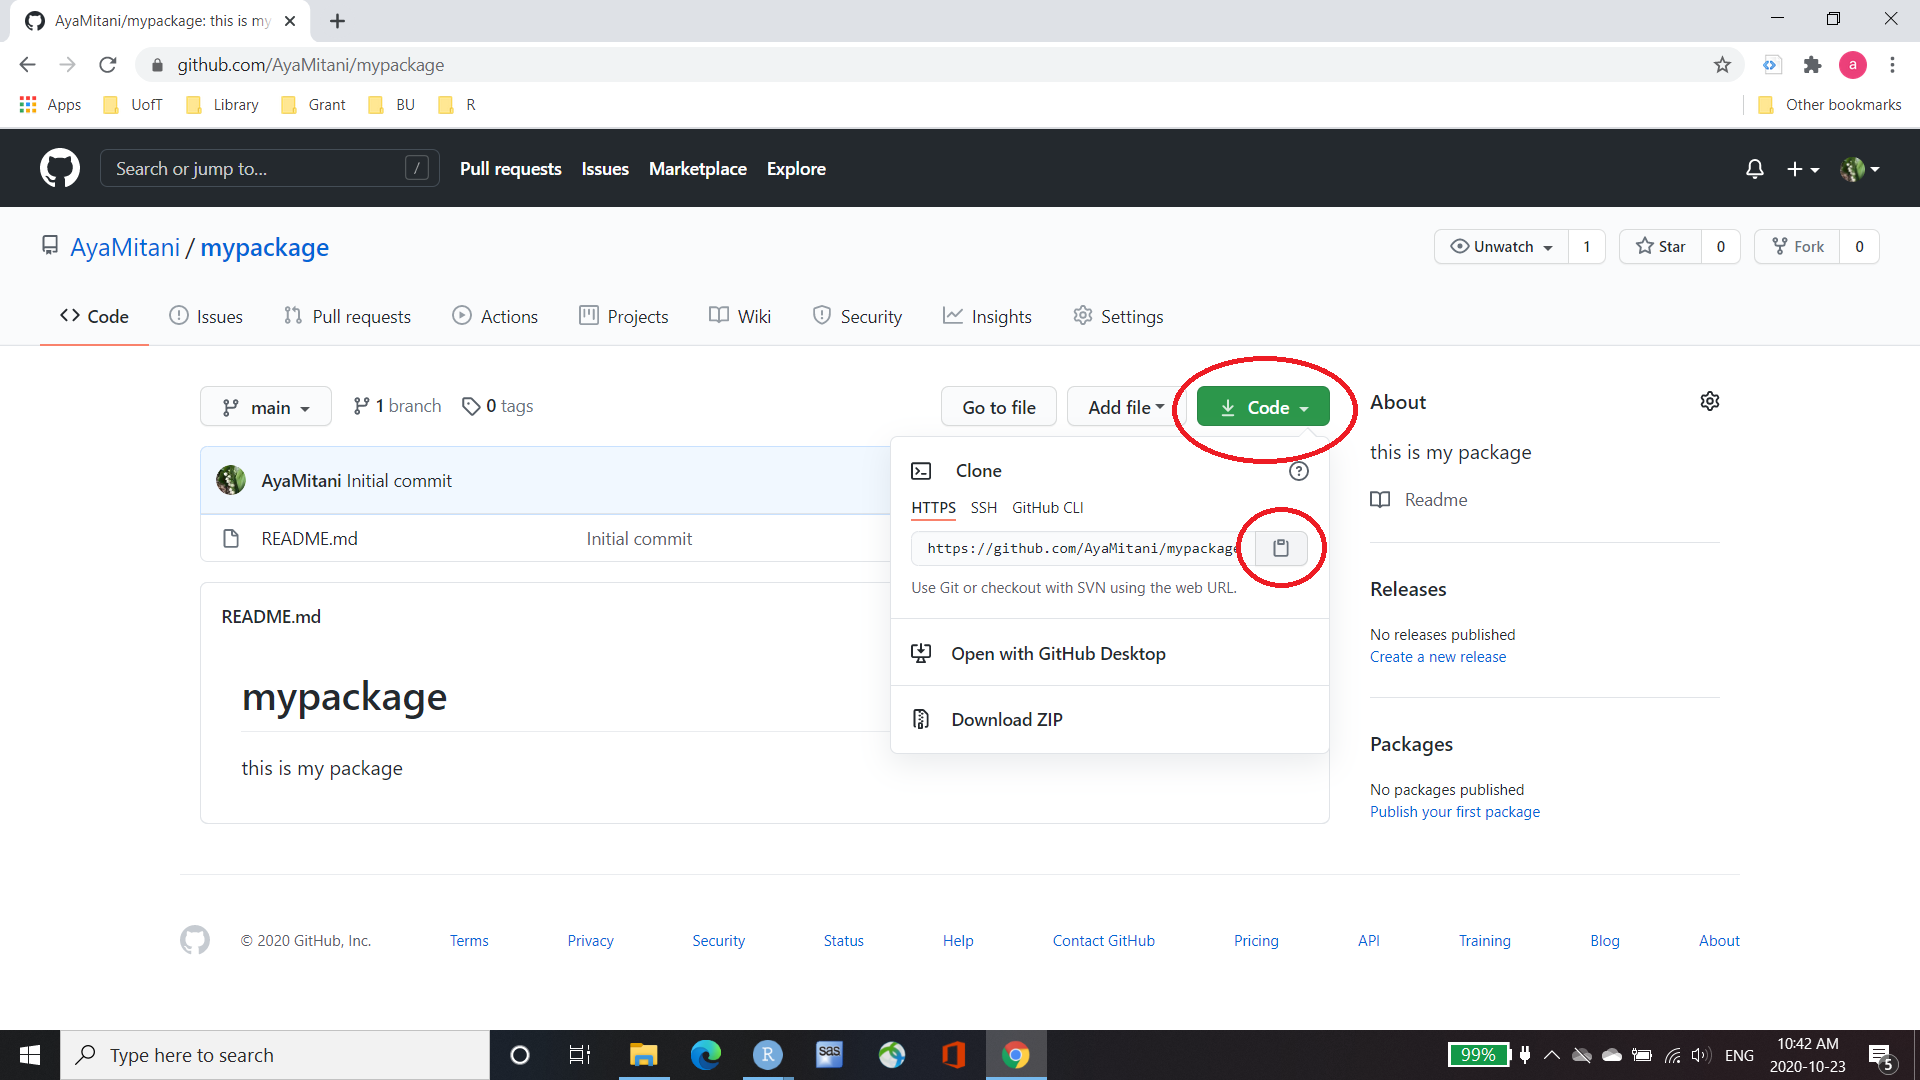
\includegraphics[scale=0.275]{slides_files/figure-beamer/GitHub_step5.png}
\end{figure}

\end{frame}

\begin{frame}[fragile]{In RStudio}
\protect\hypertarget{in-rstudio}{}

Load libraries

\begin{Shaded}
\begin{Highlighting}[]
\KeywordTok{library}\NormalTok{(devtools)}
\KeywordTok{library}\NormalTok{(here)}
\end{Highlighting}
\end{Shaded}

\end{frame}

\begin{frame}[fragile]{Turn this project into a package}
\protect\hypertarget{turn-this-project-into-a-package}{}

\begin{Shaded}
\begin{Highlighting}[]
\NormalTok{devtools}\OperatorTok{::}\KeywordTok{create}\NormalTok{(here}\OperatorTok{::}\KeywordTok{here}\NormalTok{())}
\end{Highlighting}
\end{Shaded}

This will create 3 additional files

\begin{itemize}
\tightlist
\item
  DESCRIPTION: This is where all the meta-data about your package goes.
  You can edit this file manually.
\item
  NAMESPACE: This file indicates what needs to be exposed to users for
  your R package. Do not edit this file.
\item
  R: This is where all your R code goes for your package.
\end{itemize}

\end{frame}

\begin{frame}[fragile]{Add your function}
\protect\hypertarget{add-your-function}{}

Open new R script and write your function

\begin{Shaded}
\begin{Highlighting}[]
\NormalTok{myfunc <-}\StringTok{ }\ControlFlowTok{function}\NormalTok{(x)\{}
\NormalTok{  y <-}\StringTok{ }\NormalTok{x }\OperatorTok{+}\StringTok{ }\NormalTok{x}
  \KeywordTok{return}\NormalTok{(y)}
\NormalTok{\}}
\end{Highlighting}
\end{Shaded}

\end{frame}

\begin{frame}[fragile]{Add your function}
\protect\hypertarget{add-your-function-1}{}

Include \texttt{@export} tag above your function to indicate this
function to be ``exposed'' to users.

\begin{Shaded}
\begin{Highlighting}[]
\CommentTok{#' @export}
\NormalTok{myfunc <-}\StringTok{ }\ControlFlowTok{function}\NormalTok{(x)\{}
\NormalTok{  y <-}\StringTok{ }\NormalTok{x }\OperatorTok{+}\StringTok{ }\NormalTok{x}
  \KeywordTok{return}\NormalTok{(y)}
\NormalTok{\}}
\end{Highlighting}
\end{Shaded}

\end{frame}

\begin{frame}[fragile]{Add your function}
\protect\hypertarget{add-your-function-2}{}

Also, include documentation for your function when you go
\texttt{?myfunc}. \small

\begin{Shaded}
\begin{Highlighting}[]
\CommentTok{#' This is my function.}
\CommentTok{#'}
\CommentTok{#' This function returns a value from adding the parameters.}
\CommentTok{#' @param x}
\CommentTok{#' @return y}
\CommentTok{#' @export}
\NormalTok{myfunc <-}\StringTok{ }\ControlFlowTok{function}\NormalTok{(x)\{}
\NormalTok{  y <-}\StringTok{ }\NormalTok{x }\OperatorTok{+}\StringTok{ }\NormalTok{x}
  \KeywordTok{return}\NormalTok{(y)}
\NormalTok{\}}
\end{Highlighting}
\end{Shaded}

\end{frame}

\begin{frame}[fragile]{Add your function}
\protect\hypertarget{add-your-function-3}{}

Now run

\begin{Shaded}
\begin{Highlighting}[]
\NormalTok{devtools}\OperatorTok{::}\KeywordTok{document}\NormalTok{()}
\end{Highlighting}
\end{Shaded}

\begin{itemize}
\tightlist
\item
  This will create \texttt{man} directory that includes read-only file
  \texttt{myfunc.Rd}
\item
  Note that \texttt{NAMESPACE} file has been updated
\end{itemize}

\end{frame}

\begin{frame}{Add data set}
\protect\hypertarget{add-data-set}{}

\end{frame}

\end{document}
